\chapter{Desarrollo del proyecto}

\section{Extracción y recoleccion de datos}

\subsection{Introducción}

En el siguiente apartado se expone la metodología de obtención de los datos de entrena-miento.

Las distintas versiones de MoViNets están entrenadas sobre \href{https://www.deepmind.com/open-source/kinetics}{Kinetics 600}, por lo que para reentrenar el modelo necesitamos \textit{clips} (videos) que representen los movimientos que se quieren predecir.

Si bien no existe un conjunto de datos similar aplicado específicamente a movimientos de crossfit, muchos atletas suben videos a youtube de realizando distintas pruebas y ejercicios. Partiendo de estos videos, se pueden extraer los distintos \textit{clips} (trozos) que representen los movimientos con los que reentrenar el modelo.

Todos los videos descargados pertenecen a la primera etapa de los \href{https://en.wikipedia.org/wiki/2020_CrossFit_Games}{Crossfit Games de 2020}). Este año fue algo atípico debido a la pandemia: La final de la competición se distinguió en dos etapas, una primera en formato online, y la final a la que solo pudieron acceder 10 atletas en total (5 hombres y 5 mujeres). Los videos correspondientes a la primera etapa están todos subidos a YouTube, dentro de las \href{https://www.youtube.com/c/CrossFitGamesTV/playlists}{listas de CrossFit Games}, donde todos los atletas están grabados de forma individual y con la cámara estática, lo que reduce enormemente el ruido de los datos.


\subsection{Proceso de extracción}

Para seleccionar la muestra de videos, se ha partido de 4 \textit{eventos} \footnote{Los videos corresponden a los siguientes eventos, que se pueden encontrar \href{https://games.crossfit.com/workouts/games/2020}{aquí}: \textit{Friendly Fran}, \textit{Damn Diane}, \textit{Nasty Nancy} y \textit{Awful Annie}.} que en total dan pie a 9 movimientos (ver las etiquetas en el siguiente \href{https://gist.github.com/plaguss/58091caefee6acb39ae51cbc241b3cf9/raw/labels.txt}{\textit{gist}}).

De cada \textit{evento} se han seleccionado 20 videos (10 de hombres y 10 de mujeres), de los cuales se han etiquetado 15 repeticiones de cada movimiento presente. Esto nos deja con una muestra de alrededor de 300 repeticiones por movimiento, 2700 clips.

Para descargar los videos se ha utilizado \href{https://github.com/yt-dlp/yt-dlp}{\texttt{yt-dlp}}, todos con la misma resolución (480 x 854p) en formato mp4. El siguiente script: \href{https://github.com/plaguss/tfm-misc/blob/main/scripts/download.py}{\texttt{download.py}}, se ha utilizado para las descargas de todos los videos.

El etiquetado de los videos se ha hecho con \href{https://supervise.ly/}{\textit{Supervisely}} \footnote{Tras probar otras alternativas como \href{https://labelstud.io/}{\textit{LabelStudio}}, \textit{Supervisely} facilita enormemente seleccionar rangos de frames por medio de atajos del teclado.}.
Una vez se ha etiquetado un video, \textit{Supervisely} genera un \texttt{json} con las anotaciones correspondientes al movimiento y los frames en los que se produce.

Para obtener cada uno de los clips se ha utilizado \href{https://github.com/plaguss/tfm-misc/blob/main/scripts/ffmpeg-split.py}{\texttt{ffmpeg-split.py}} \footnote{Este script pertenece al siguiente \href{https://github.com/c0decracker/video-splitter}{repositorio}.}. Las anotaciones se tranforman a un formato que \texttt{ffmpeg-split.py} pueda utilizar por medio de \href{https://github.com/plaguss/tfm-misc/blob/main/scripts/manifester.py}{\texttt{manifester.py}}.

La figura \ref{data_extraction_process} resume el proceso para la obtención de los datos\footnote{Todos los scripts utilizados para la la extracción de los datos se encuentran \href{https://github.com/plaguss/tfm-misc/tree/main/scripts}{aquí}.}.


\begin{figure}[H]
    \centering
		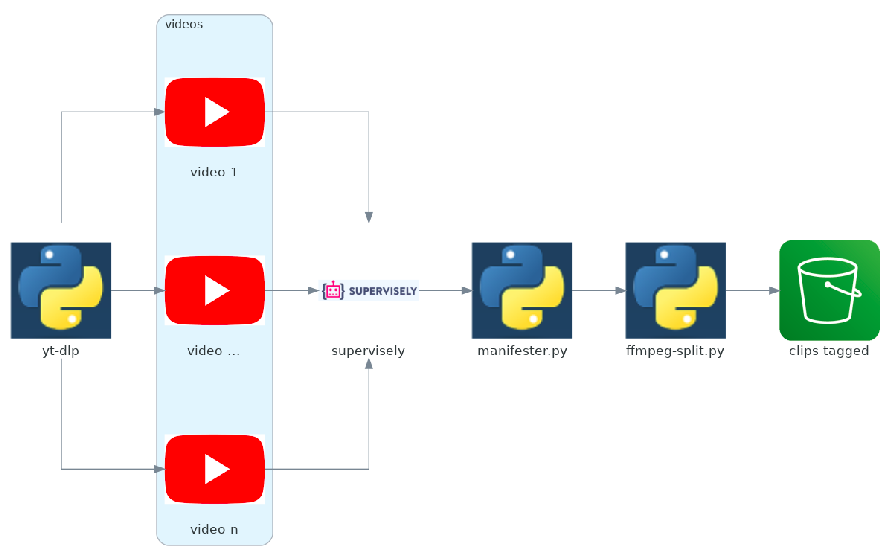
\includegraphics[width=\textwidth]{figs/data_extraction_process_.png}
\caption{Proceso de extración de datos}\label{data_extraction_process}
\end{figure}

\subsection{Datos obtenidos}

Meter tablas resumen de frames y segundos de los vídeos.
\begin{table}[htbp]
\centering
\caption{Estadísticos descriptivos de los frames y duración de los clips}
\label{table_descriptive_stats}
\begin{tabular}{l|lc|lc}
\toprule
{} & \multicolumn{2}{c|}{\textbf{Frames}} & \multicolumn{2}{c}{\textbf{Duración (s)}} \\
{} &    Media & Desviación típica &        Media & Desviación típica \\
\midrule
\textbf{thruster}          &  27.7396 &            4.5060 &       0.9419 &            0.1274 \\
\textbf{chest-to-bar}      &  21.0478 &            7.4233 &       0.7196 &            0.2569 \\
\textbf{double-unders}     &  14.5880 &            1.2740 &       0.4841 &            0.0439 \\
\textbf{ghd}               &  58.9732 &            5.5611 &       1.9654 &            0.1860 \\
\textbf{power clean}       &  67.3567 &           13.0092 &       2.2448 &            0.4337 \\
\textbf{deadlift}          &  24.1229 &            7.1950 &       0.8048 &            0.2395 \\
\textbf{shspu}             &  43.2100 &           15.1247 &       1.4412 &            0.5055 \\
\textbf{ohs}               &  31.9767 &            5.4303 &       1.0664 &            0.1799 \\
\textbf{bar-facing burpee} &  62.0233 &           10.0239 &       2.0688 &            0.3340 \\
\textbf{TOTAL}             &  39.0042 &           7.7275  &       1.3041 &            0.2563 \\
\bottomrule
\end{tabular}
\end{table}



\section{Experimentación con deep learning}

\subsection{Introducción}

En esta sección se explica el modelo seleccionado, el tratamiento aplicado a los datos, el entrenamiento del modelo y los resultados obtenidos.

Existe más de una implementación de los modelos de MoViNets como se puede ver en \href{https://paperswithcode.com/paper/movinets-mobile-video-networks-for-efficient}{\textit{Papers with code}}, pero dado que los autores del \textit{paper} original han desarrollado el mismo utilizando \texttt{tensorflow}, y el repositorio está expuesto de manera pública junto con todos los datos entrenados, se ha decidido utilizar la versión que se puede ver en el \href{repositorio oficial}{https://github.com/tensorflow/models/tree/master/official/projects/movinet} de \textit{MoViNets}.

\subsection{Preprocesado de los datos}

De cara a construir la pipeline para el entrenamiento del modelo, se ha utilizado la API de \href{https://www.tensorflow.org/api_docs/python/tf/data/Dataset}{\texttt{tf.data.Dataset}} ya que permite la ingesta de un conjunto potencialmente grande de datos, así como el procesamiento de los mismos.

La forma más eficiente (BUSCAR REFERENCIA) de leer los videos en el \texttt{Dataset} es escribirlos como \href{https://www.tensorflow.org/api_docs/python/tf/data/TFRecordDataset}{\texttt{tf.data.TFRecordDataset}}, 
\texttt{tf.data.TFRecordDataset}
(REVISAR PARA QUE SALGA LA REFERENCIA)
para lo cuál se deben transformar los videos en formato mp4 a \texttt{tfrecords}. (INSERTAR REFERENCIA A movinets\_helper/writer.py, Y LOS DISTINTOS EJEMPLOS)

Al introducir los videos, se cambia el tamaño para igualarlo al utilizado en el entrenamiento original, 224x224p, y se escalan los valores para que se encuentren en el rango $[0, 1]$.

Para homogeneizar los datos de entrada se ha decidido fijar al número de frames para todos los videos a 10 ($\bar{f}=10$)(BUSCAR REFERENCIA A LOS DATOS UTILIZADOS EN EL PAPER ORIGINAL). Debido a que los vídeos en este conjunto de datos son más cortos que los utilizados en el caso de \textit{Kinetics 600}, se ha seleccionado el número de frames como $\bar{f} = \min_v f_{v}$, donde $f_v$ es el número de frames del vídeo $v$. El menor número de frames corresponde a uno de los vídeos de \textit{double-unders}. Para aquellos vídeos con un número de frames mayor que $\bar{f}$, se seleccionan $\bar{f}$ frames equiespaciados.

En la siguiente imagen podemos ver el ejemplo de uno de los \textit{clips} que entran en la muestra de entrenamiento. Se trata de un \textit{power clean}, donde se pueden ver las distintas imágenes que componen el \textit{clip}.

\begin{figure}[H]
    %\centering
    \centerline{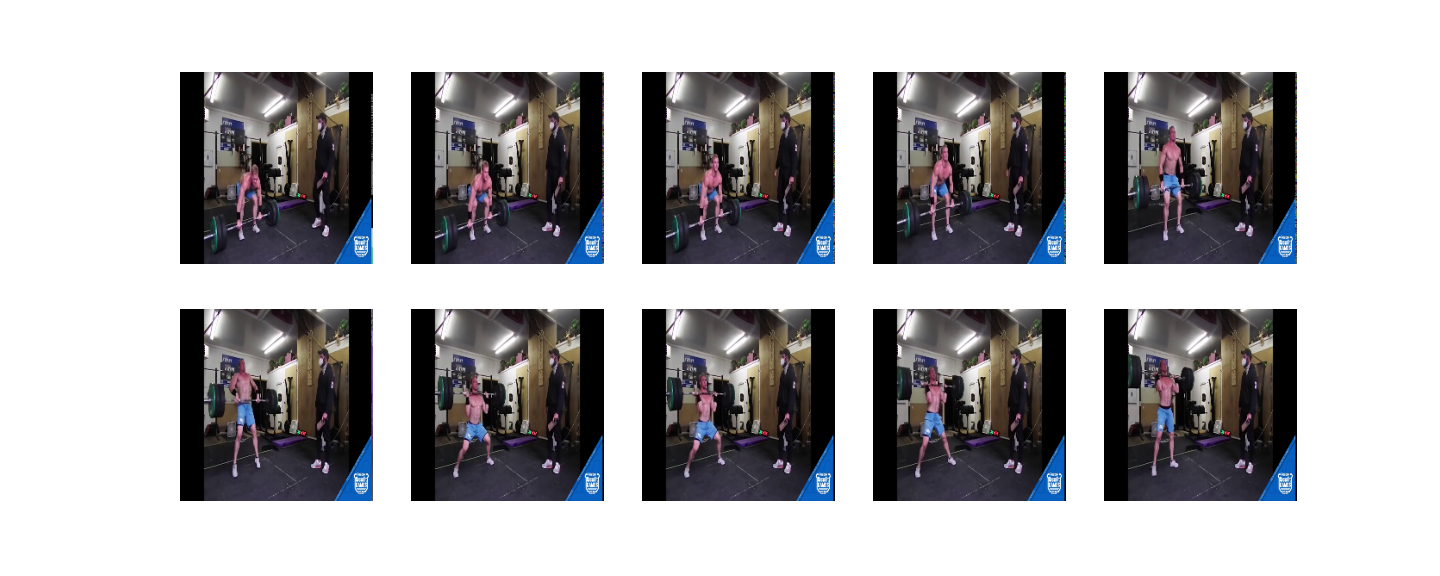
\includegraphics[width=1.25\linewidth]{figs/frames.png}}
\caption{Frames de una muestra de \textit{power clean} de la pipeline de entrenamiento}\label{frames}
\end{figure}

\subsection{Experimentos realizados y resultados}

El modelo se ha entrenado en \href{https://colab.research.google.com/?hl=es}{\textit{Google Colab}} con \textit{Tensorflow 2}. El modelo seleccionado ha sido MoViNets A2 Base\footnote{No ha sido posible hacer fine-tuning del modelo Stream debido a un error en los modelos guardados, ver \href{https://github.com/tensorflow/models/issues/10730}{issue 10730}.}, ya aunque sea necesario utilizar GPU para el fine-tuning, es el modelo más grande (y con mejor capacidad predictiva) que permite hacer inferencia con CPU en un tiempo razonable (BUSCAR REFERENCIA DE LOS AUTORES).

Los hiperparámetros del modelo son los mismos utilizados en el paper original\footnote{Ver apartado \textit{B.1 More Details of the Architectures and Training} de METER BIBLIOGRAFÍA PARA EL PAPER}, con un tamaño de batch igual a 8\footnote{El tamaño del batch seleccionado es el mismo utilizado por los autores en el tutorial a modo de ejemplo sobre el dataset UCF101.}.

La muestra se divide en un $80\%$ (2164 clips) para training, y un $20\%$ (541 clips) para test, donde los ejemplos se distribuyen de manera balanceada (ver figura \ref{sample_sizes}).

\begin{figure}[H]
    \centering
		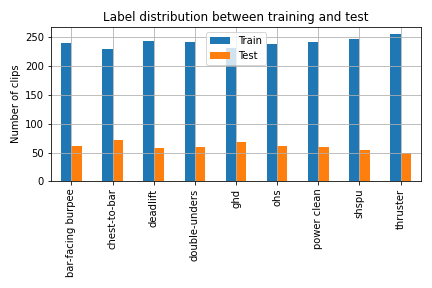
\includegraphics[width=\textwidth]{figs/sample_sizes.png}
\caption{Distribución de las etiquetas entre la muestra de entrenamiento y test}\label{sample_sizes}
\end{figure}

El modelo se ha entrenado por 10 epochs, evaluando top 1 y top 5 accuracy, obteniendo un accuracy de 0.9995 y 1 en entrenamiento y test respectivamente, como podemos observar en la siguiente imagen extraída de \textit{tensorboard.dev}:

\begin{figure}[H]
    \centering
		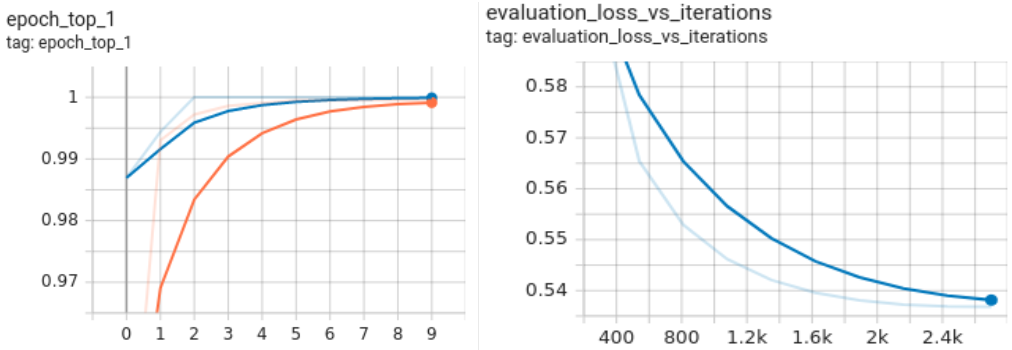
\includegraphics[width=\textwidth]{figs/tensorboard_training.png}
\caption{Top 1 categorial accuracy por epoch y loss frente por número de iteraciones}\label{training}
\end{figure}

El modelo base generaliza a un gran número de movimientos, incluyendo algunos movimientos similares\footnote{Por ejemplo, entre las  \href{https://raw.githubusercontent.com/tensorflow/models/f8af2291cced43fc9f1d9b41ddbf772ae7b0d7d2/official/projects/movinet/files/kinetics_600_labels.txt}{labels de Kinetics 600} se encuentran \textit{squat}, \textit{clean and jerk} o \textit{snatch weight lifting}.} , lo que puede facilitar seguir aprendiendo algunos de movimientos similares.

Por otro lado, los videos en este caso, aunque se han seleccionado de una muestra distinta de atletas, todos ellos son atletas de élite en su deporte, por lo que la ejecución de los movimientos son muy similares entre si, lo que facilita aprender a clasificar los mismos.

Los resultados del entrenamiento se pueden ver en de forma interactiva en el siguiente enlace a \href{https://tensorboard.dev/experiment/UXyupsnMQ2S74vdul3vdbw/#scalars}{\textit{Tensorboard.dev}}.


\subsection{Evaluación de los resultados}

A la hora de evaluar los resultados, empezamos analizando el heatmap de la matriz de confusión. Como se vio al analizar el accuracy en la muestra de test, todos los movimientos se clasifican bien (ver imagen \ref{app_3}).

\begin{figure}[H]
    \centering
		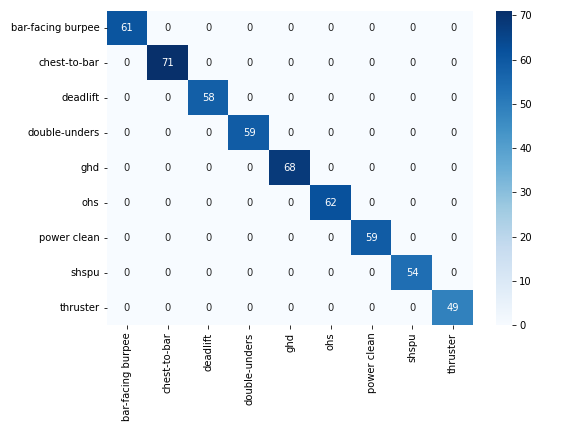
\includegraphics[width=\textwidth]{figs/heatmap_confusion.png}
\caption{Heatmap de la matriz de confusión para la muestra de test.}\label{app_3}
\end{figure}

Con vistas a proporcionar un análisis más robusto en caso de extender el modelo a un mayor número de movimientos o muestras de distintos atletas, puede ser útil la información que proporciona el heatmap de la figura \ref{heatmap_correlations}. La construcción de este gráfico se hace de la siguiente forma:

Partiendo de las probabilidades asignadas a cada vídeo en el período de test, se fija para cada movimiento (cada \textit{label} correcta) y se calculan las correlaciones. Se selecciona la correlación (de Pearson) con el movimiento correctamente etiquetado, y se concatenan todos los vectores columna, de forma que obtenemos una matriz cuadrada. Estas correlaciones ayudan a ver cuáles son los movimientos que más se "confunden" entre si. Dado que las probabilidades deben sumar 1, aquellos movimientos con una correlación negativa más cercana a 1, son aquellos en los que se puede observar una mayor intercambio de probabilidades en la predicción.

\begin{figure}[H]
    \centering
		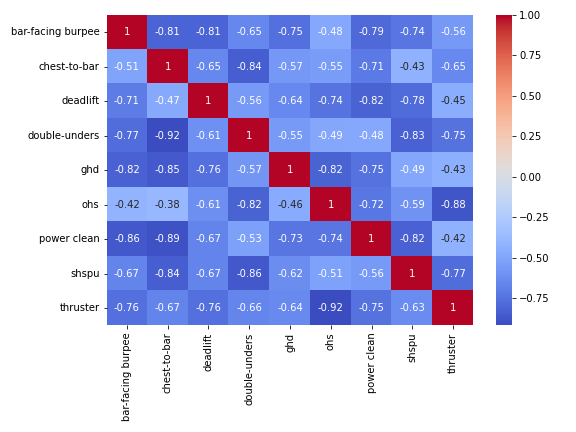
\includegraphics[width=\textwidth]{figs/heatmap_correlations.png}
\caption{Heatmap de correlación entre probabilidades. Para los clips clasificados como $j$, la celda $(i, j)$ representa la correlación entre las probabilidades de predecir el movimiento $i$ y el movimiento $j$.}\label{heatmap_correlations}
\end{figure}

Por ejemplo, si nos fijamos en la columna que corresponde a \textit{ohs}, vemos que el mayor coeficiente de correlación es de $-0.92$, con \textit{thruster}. Esto tiene sentido si se tiene en cuenta que en ambos movimientos, la barra parte de una sentadilla y acaba con la barra bloqueada por encima de la cabeza.

Por último, se puede ver en la siguiente tabla las probabilidades medias y desviación estándar obtenidas para cada movimiento correctamente etiquetado. Esto nos permite ver cuáles son los movimientos que se predicen con una mayor confianza, como en este caso los \textit{double-unders}, o los que menos, los \textit{ohs}. Las probabilidades que dan lugar a esta tabla se pueden ver en \ref{Probabilidades}.


\begin{table}[H]
\centering
\caption{Estadísticos principales }
\label{table_probabilities}
\begin{tabular}{lcc}
\toprule
{} &   Media &  Desviación típica \\
\midrule
double-unders     &  0.8921 &             0.0748 \\
ghd               &  0.8904 &             0.0533 \\
bar-facing burpee &  0.8876 &             0.0756 \\
thruster          &  0.8838 &             0.0590 \\
deadlift          &  0.8746 &             0.0796 \\
shspu             &  0.8731 &             0.0843 \\
chest-to-bar      &  0.8552 &             0.1282 \\
power clean       &  0.8443 &             0.0851 \\
ohs               &  0.8438 &             0.1163 \\
\bottomrule
\end{tabular}
\end{table}


\section{Cloud y despliegue de la aplicación}

En el siguiente apartado se presenta la aplicación para clasificar movimientos de crossfit, la arquitectura elegida así como su funcionamiento para un ejemplo en concreto.

\subsection{Introducción}

Para la explotación del modelo se ha elegido desplegar una aplicación en AWS desarrollada en Plotly Dash. Un usuario solo necesita subir un video en formato mp4, y recibir a cambio las predicciones del mismo. En los siguientes apartados se puede ver la arquitectura de la aplicación en la nube y los resultados obtenidos.

\subsection{Arquitectura cloud}

A continuación se puede ver en la figura \ref{cloud_diagram} el diagrama de la aplicación desplegada en AWS.

El punto de entrada para un usuario es la aplicación desplegada en \href{https://aws.amazon.com/es/ec2/}{\textit{EC2}}, cuyo código se puede ver en el repositorio \href{https://github.com/plaguss/movinets_dash_app}{\texttt{movinets\_dash\_app}}.

La app está desarrollada en \href{https://plotly.com/dash/}{\textit{Dash}}, y ofrece la funcionalidad justa para subir un video en formato mp4 (y mostrarlo), obtener las probabilidades asociadas a cada movimiento, y mostrar ejemplos de los movimientos para los que se ha entrenado el modelo.

Se pueden distinguir dos bloques:
%
\begin{itemize}%
%
\item \textit{App pipeline}.
Por un lado tenemos la aplicación con la que interactúa el usuario.
Se parte de un repositorio público en github que contiene el código del front end. Por medio de \href{https://aws.amazon.com/es/codepipeline/}{AWS CodePipeline} y \href{https://aws.amazon.com/es/codedeploy/}{AWS CodeDeploy} se automatiza el despliegue de la misma en una instancia de \textit{EC2}, que viene desencadenado por medio de un \texttt{git push} a la rama master del repositorio.

\item \textit{Model predictions}.
Al subir un video, este se puede mandar a predecir (solo se reproduce en pantalla por defecto). El proceso en este caso contempla la interacción con el modelo por medio de una función \href{https://aws.amazon.com/es/lambda/}{\textit{AWS Lambda}}. Debido a las restricciones de tamaño de lambda, no es posible desplegar el código de la misma simplemente comprimiendo las dependencias ya que tensorflow por si solo excede el límite. El código de la lambda \href{https://github.com/plaguss/tfm-misc/tree/main/lambda_aws}{(ver aquí)} se debe empaquetar en Docker y subir la imagen a \href{https://aws.amazon.com/es/ecr/}{ECR}. La lambda se encarga por tanto de leer el video, cargar el modelo almacenado en S3, transformar el video al formato adecuado, y devolver las probabilidades asociadas al mismo.

\end{itemize}


\begin{figure}[H]
    \centering
		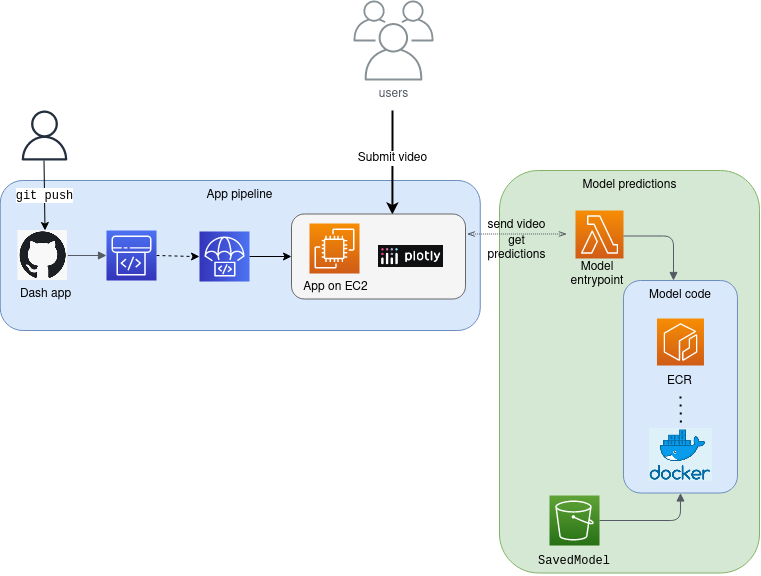
\includegraphics[width=\textwidth]{figs/cloud_diagram.png}
\caption{Diagrama Cloud}\label{cloud_diagram}


\end{figure}

\subsection{Resultado y funcionamiento}

A continuación se puede ver una serie de capturas de la app desplegada. La figura \ref{app_1} muestra la pantalla inicial de la app. La pestaña principal \textit{Clip prediction} permite cargar el vídeo arrastrando el archivo o buscándolo por su nombre. La pestaña secundaria \textit{Examples} permite ver ejemplos de los movimientos. 

\begin{figure}[H]
    \centering
		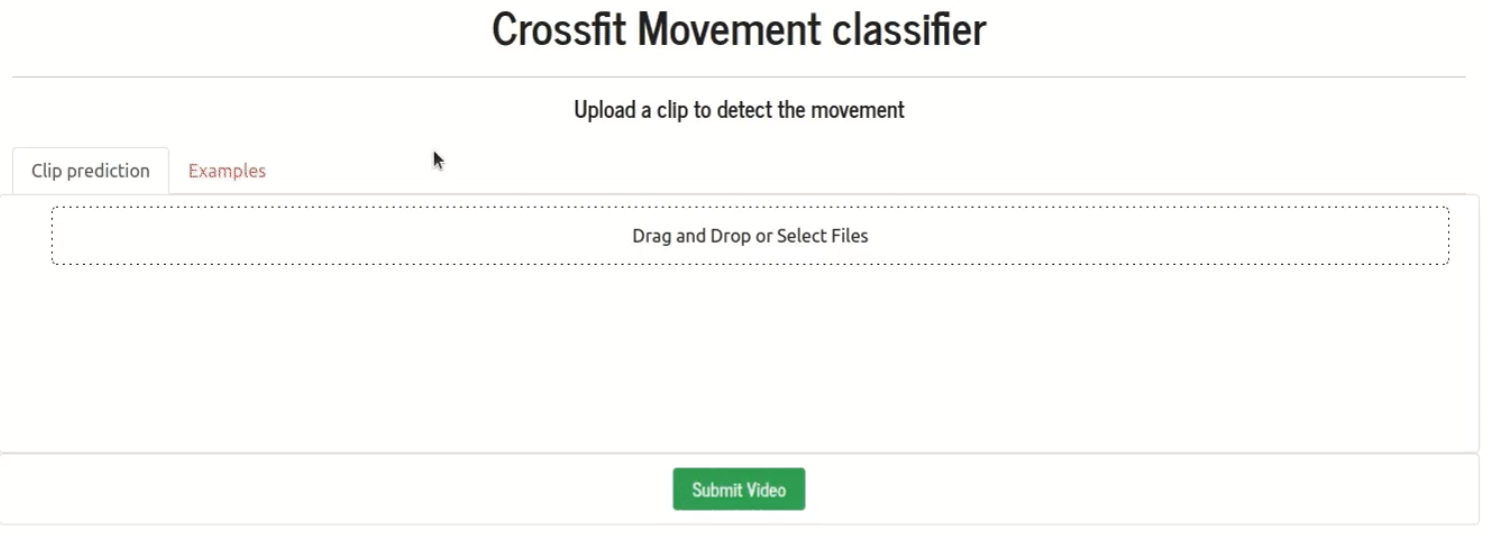
\includegraphics[width=\textwidth]{figs/app_1.png}
\caption{App: Estado inicial}\label{app_1}
\end{figure}

Una vez se ha subido un clip, este se reproduce de forma automática (figura \ref{app_2}). Para poder obtener las probabilidades asociadas al movimiento en cuestión habría que pulsar el botón \textit{Submit Video}, que envía el contenido a la función lambda.

\begin{figure}[H]
    \centering
		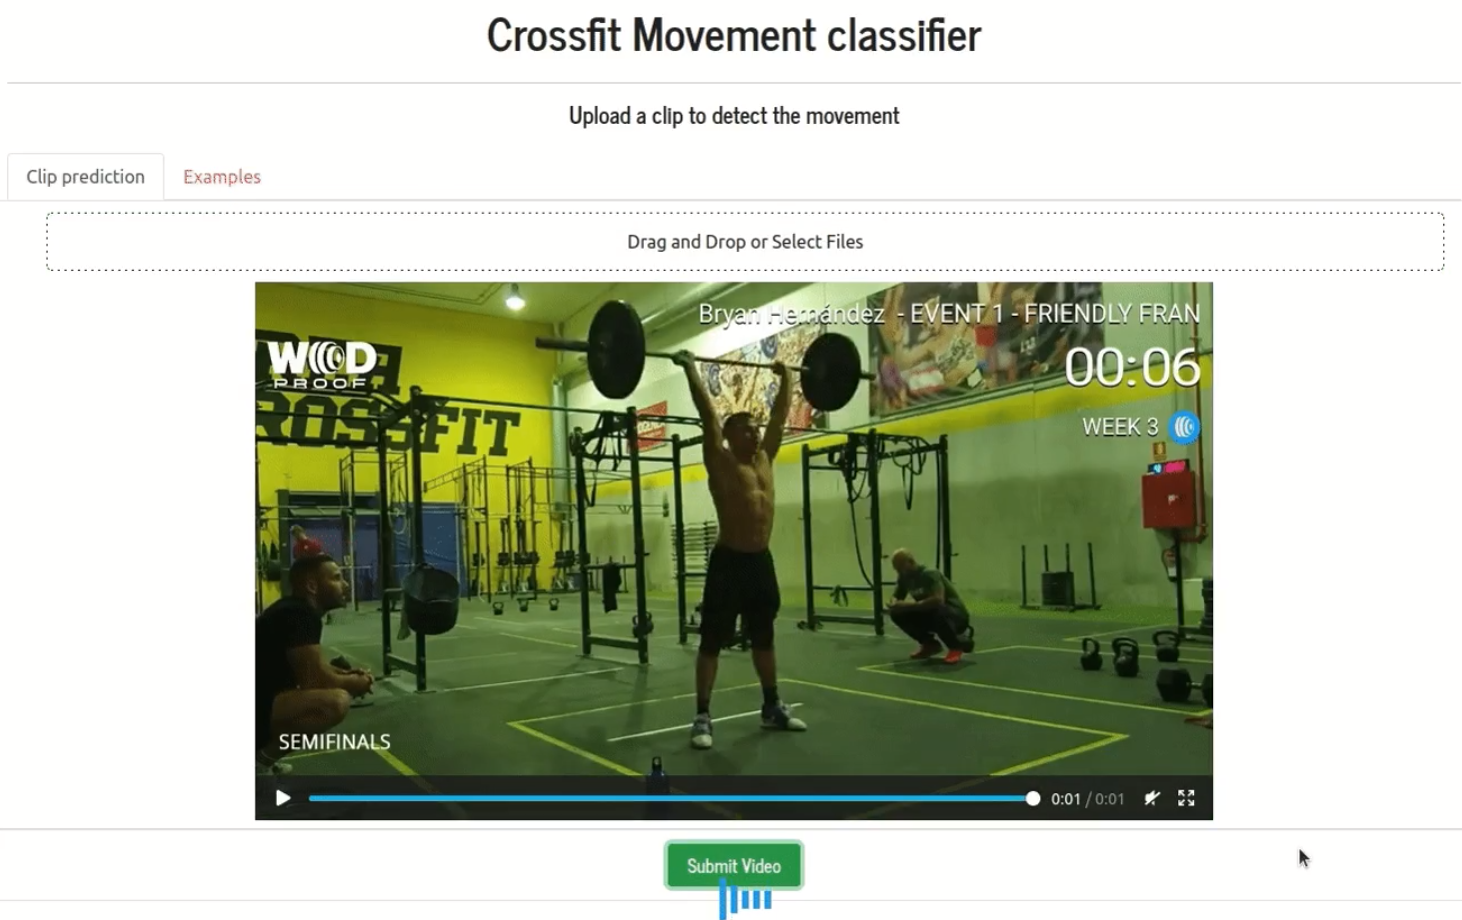
\includegraphics[width=\textwidth]{figs/app_2.png}
\caption{App: Video cargado}\label{app_2}
\end{figure}

Tras obtener la predicción del modelo, justo debajo aparece la tabla con los 5 movimientos más probables y la probabilidad asociada a cada uno de ellos, ordenados de mayor a menor, como muestra la figura \ref{app_3}.

\begin{figure}[H]
    \centering
		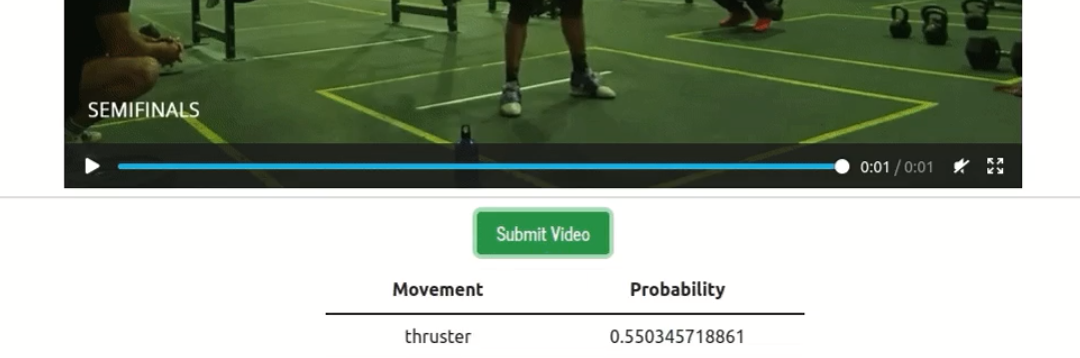
\includegraphics[width=\textwidth]{figs/app_3.png}
\caption{App: Extracto de tabla de predicciones}\label{app_3}
\end{figure}

Si bien los vídeos se han entrenado con un máximo de 10 frames, en este caso el vídeo se pasa al modelo sin hacer un muestreo de los mismos. Aunque solo se ha comprobado para unos pocos ejemplos de los vídeos completos, las probabilidades se ven afectadas, pero la ordenación de los mismos se mantiene.

El tiempo aproximado para obtener las predicciones asociadas a un clip es de alrededor de 14 segundos para un thruster, que es un movimiento relativamente corto (ver tabla \ref{table_descriptive_stats}), por lo que clasificar los movimientos es lento.

Como alternativas para ganar velocidad, se podría reducir el tamaño del modelo para mejorar la latencia de la CPU, limitando el número de posiciones decimales por ejemplo, un procedimiento conocido como \href{https://www.tensorflow.org/lite/performance/post_training_quantization}{\textit{post-training quantization}}. Los autores originales ofrecen versiones del mismo ya entrenadas para este caso \href{https://tfhub.dev/google/collections/movinet/1}{aquí}.

Existen otras alternativas. Se podría hacer un muestreo del vídeo de la misma forma que se hace durante la pipeline de entrenamiento (cabe recordar que durante el entrenamiento, el modelo solo utiliza 10 frames de cada vídeo), con lo que la información a procesar disminuiría. Otra opción sería entrenar un modelo de menor complejidad, ya sea la versión a0 o a1, ya que el accuracy actual ya es excepcionalmente alto.



